\documentclass[11pt]{article}
\usepackage[utf8x]{inputenc}
\usepackage[croatian]{babel}
\usepackage{amsmath}
\usepackage{amsthm}
\usepackage{amsfonts}
\usepackage{color}
\usepackage{longtable}
\usepackage{tabu}
\usepackage{tikz}
\usepackage{extpfeil}
\usepackage{hyperref}
\usepackage{listings}

\newextarrow{\xbigtoto}{{20}{20}{20}{20}}
{\bigRelbar\bigRelbar{\bigtwoarrowsleft\rightarrow\rightarrow}}

\definecolor{codegray}{gray}{0.9}
\newcommand{\category}[1]{\textbf{\emph{#1}}}
\newcommand{\codei}[1]{
  {\lstinline[basicstyle=\ttfamily]{#1}}
}
\newcommand{\code}[1]{
  \begin{align*}
    \texttt{#1}
  \end{align*}
  }
\theoremstyle{definition}
\newtheorem{definition}{Definicija}
\newtheorem{primjer}{Primjer}
\newtheorem{koloral}{Koloral}
\newtheorem{teorem}{Teorem}

\begin{document}
  %%%%%%%%%%%%%%%%%%%%%%%%%%%
  %% Definicija Kategorije %%
  %%%%%%%%%%%%%%%%%%%%%%%%%%%
  \section{Kategorije}
  Teorija kategorije proucava "objekte" i "preslikavanja" izmedu
  njih. Objekti i preslikavanja su primitivni objekti u teoriji kategorija i
  njih ne definiramo. Objekti ne moraju biti kolekcije elemenata i
  preslikavanja ne moraju biti funkcije na skupovima.
  U ovom poglavlju definiramo kategorije i detaljno raspisujemo nekoliko
  primjera.
  \begin{definition}
    Kategorija $G$ sastoji se od:
    \begin{itemize}
      \item klase objekata $Obj$
      \item klase strelica $Arw$
      \item preslikavanje $Arw \xrightarrow{source} Obj$
      \item preslikavanje $Arw \xrightarrow{target} Obj$
      \item preslikavanje (identiteta) $Obj \xrightarrow{id} Arw$ takvog da
      za $B \xrightarrow{id} id_B$ vrijedi:
        \begin{equation}
          target(id_B) = source(id_B) = B
        \end{equation}
      \item preslikavanje (kompozicija) $Arw \times Arw \xrightarrow{\circ}
      Arw$ takvog da za \\ $(f, g) \xrightarrow{\circ} f \circ g$ vrijedi:
        \begin{align}
          source(f) &= target(g) \\
          source(f \circ g) &= source(g) \\
          target(f \circ g) &= target(f)
        \end{align}
    \end{itemize}
    Preslikavanje identiteta ($id$) i kompozicija ($\circ$) moraju
    zadovoljavati:
    \begin{itemize}
      \item svojstvo identiteta: za svaku strelicu $A \xrightarrow{f} B$ vrijedi:
        \begin{align}
          id_B \circ f = f = f \circ id_A
        \end{align}
      \item svojstvo asocijativnost: za sve strelice $A \xrightarrow{f} B
      \xrightarrow{g} C \xrightarrow{h} D$ vrijedi:
        \begin{align} \label{def:kat_assoc}
          (h \circ g) \circ f = h \circ (g \circ f)
        \end{align}
    \end{itemize}
  \end{definition}
  Kada zelimo posebno naglasiti kojoj kategoriji pripadaju strelice i objekti
  onda cemo umjesto $Obj$ i $Arw$ pisati $Obj_G$ i $Arw_G$.
  Za $A, B \in Obj_G$ skup svih strelica sa $A$ u $B$ oznacavamo sa
  \category{G}$[A, B]$.
  Sada cemo detaljno raspisati nekoliko primjera kategorija.

  %%%%%%%%%%%%%%%%%%%%
  %% Mon Kategorija %%
  %%%%%%%%%%%%%%%%%%%%
  \begin{primjer}
    \textbf{Monoid} je uredena trojka $(M, \cdot_M, 1_M)$ gdje je $M$ skup, $1_M
    \in M$, $\cdot_M$ binarna operacija na $M$ za koju vrijedi da za svaki $a, b, c \in M$:
    \begin{equation*}
      (a \cdot_M b) \cdot_M c = a \cdot_M (b \cdot_M c)
    \end{equation*}
    \begin{equation*}
      1_M \cdot_M a = a = a \cdot_M 1_M
    \end{equation*}
    Neutralni element $1_M$ i binarnu operaciju $\cdot_M$ cemo uglavnom pisati
    kao $1$ i $\cdot$ osim ako nece biti jasno iz konteksta na kojem monoidu
    su defnirani.
    Kada monoid promatramo kao kategoriju tada su objekti skupovi, a
    za dva monoida $M, N$ definiramo strelicu $M \xrightarrow{\delta} N$ kao
    funkciju za koju vrijedi da za svaki $a, b \in M$ vrijedi:
    \begin{equation*}
      \delta(a \cdot b) = \delta(a) \cdot \delta(b)
    \end{equation*}
    \begin{equation*}
      \delta(1) = 1
    \end{equation*}
    i zovemo ju \textbf{morfizam}.
    Pokazimo da je kompozicija dva morfizma morfizam.
    Neka su $a, b \in Obj_M$ i $M \xrightarrow{f} N \xrightarrow{g} P$, tada vrijedi:
    \begin{equation*}
      (g \circ f)(a \cdot b) = g(f(a \cdot b)) = g(f(a) \cdot f(b)) = g(f(a))
      \cdot g(f(b)) = (g \circ f)(a) \cdot (g \cdot f)(b)
    \end{equation*}
    Za monoid $M$ definiramo identitetu $id_M$ kao standardnu funkciju
    identiteta, tj. za svaki $a \in Obj_M$ vrijedi:
    \begin{equation*}
      id_M(a) = a
    \end{equation*}
    Pokazimo sada da tako definiran strelice na monoidu zadovoljavaju
    svojstvo identiteta i asocijativnosti (\ref{def:kat_assoc}) za kategorije.
    Neka je $a \in Obj_M$ i $M \xrightarrow{f} N$, tada vrijedi:
    \begin{equation*}
      (id_N \circ f)(a) = id_N(f(a)) = f(a) = f(id_M(a)) = (f \circ id_M)(a)
    \end{equation*}
    te je svojstvo identiteta zadovoljeno.
    Neka su $M, N, P, R$ monoidi, $M \xrightarrow{f} N \xrightarrow{g} P \xrightarrow{h} R$
    i $a \in Obj_M$, tada vrijedi:
    \begin{equation*}
      ((h \circ g) \circ f)(a) = h(g(f(a))) = (h \circ (g \circ f))(a)
    \end{equation*}
    zbog asocijativnosti kompozicije funkcija te monoide mozemo promatrati kao
    kategorije. Kategoriju monoida oznacavamo sa \category{Mon}.
  \end{primjer}

  %%%%%%%%%%%%%%%%%%%%
  %% Pos Kategorija %%
  %%%%%%%%%%%%%%%%%%%%
  \begin{primjer}
    Neka je $S$ skup i $\leq_S \subseteq S \times S$ relacija na $S$. Uredeni par $(S,
    \leq_S)$ zovemo \textbf{parcijalno uredeni skup} ako za svaki $a, b, c \in S$
    vrijedi:
    \begin{itemize}
      \item $a \leq_S a$ (refleksivnost)
      \item ako $a \leq_S b$ i $b \leq_S a$ tada $a = b$ (anti-simetricnost)
      \item ako $a \leq_S b$ i $b \leq_S c$ tada $a \leq_S c$ (tranzitivnost)
    \end{itemize}
    Radi kraceg zapisa pisati cemo samo $\leq$ umjesto $\leq_S$ i
  govoriti o parcijalno uredenom skupu $S$ gdje je implicitno definirna
  binarna relacija $\leq$.
  Neka su $S, R$ dva parcijalno uredena skupa i neka je $R \xrightarrow{f} S$
  preslikavanje za koje vrijedi da za svaki $a, b \in S$ vrijedi:
  \begin{equation*}
    a \leq b \implies f(a) \leq f(b)
  \end{equation*}
  Tada kazemo da je $f$ \textbf{monotono preslikavanje}.
  Pokazimo da su monotona preslikavanja zatvorena na kompoziciju.
  Neka su $S \xrightarrow{f} R \xrightarrow{g} Q$ monotona preslikavanja i $a,
  b \in S$ takva da $a \leq b$. Tada vrijedi:
  \begin{equation*}
    a \leq b \implies f(a) \leq f(b) \implies g(f(a)) \leq g(f(b))
  \end{equation*}
  tj.
  \begin{equation*}
    a \leq b \implies (g \circ f)(a) \leq (g \circ f)(b)
  \end{equation*}
  Identiteta na parcijalnu uredenom skupu $S$ je definirana kao standardna
  funkcijska identiteta. Kao i u prethodnom primjeru pokaze se da vrijedi:
  \begin{equation*}
    (id_R) \circ f = f = f \circ id_S
  \end{equation*}
  \begin{equation*}
    (h \circ g) \circ f = h \circ (g \circ f)
  \end{equation*}
  pa mozemo govoriti u kategoriji \category{Pos} gdje su objekti parcijalno
  uredeni skupovi a strelice monotona preslikavanja.
  \end{primjer}
  %%%%%%%%%%%%%
  %% Haskell %%
  %%%%%%%%%%%%%
  Haskell je funkcijski programski jezik nazvan po logicaru Haskellu Curryiu. U
  Haskellu \textbf{tip} intuitivno mozemo shvatiti kao skup, npr.
  \category{Char} je skup svih Unicode znakova (\codei{'A'},
  \codei{')'}, \codei{'^'}), \category{Bool} sadrzi samo dva elementa
  \codei{\{True, False\}},  \category{Integer} je beskonacni skup koji sadrzi
  sve cijele brojeve.
  Kada u Haskellu zapisamo da je $x$ Integer, tj:
  \code{
    x :: Integer
  }
  to znaci da je $x$ element skupa cijelih brojeva.
  Haskellove funkcije ne mozemo poistovjetiti sa matematickim funkcijama jer
  Haskellove funkcije trebaju izvrsiti neki kod - sto nije problem ukoliko se
  moze doci do rezultata u konacno mnogo koraka, ali ponekad to nije tako. Zbog "Halting
  problema"\footnote{Ako je zadan program i ulaz za taj program, odredite hoce
    li racunanje tog program stati.
    \url{http://mathworld.wolfram.com/HaltingProblem.html}} ne mozmo se
  ograniciti samo na funkcije kod kojih se moze doci do rezultata u konacno
  mnogo koraka pa se u svaki Haskellov tip dodaje posebna vrijednost: ⊥ (dno).
  Ta posebna vrijednost oznacava da racunanje nece stati, pa tako funkciju $f:
  Bool \to Bool$  u Haskellu definirana sa:
  \code{
    f :: Bool -> Bool
  }
  moze vratiti \codei{True}, \codei{False} ili ⊥. Funkcije koje mogu vratiti ⊥
  zovemo parcijalne funkcije.
  Zbog specijalnog znaka ⊥ kategoriju Haskellovih funkcija i tipova razlikujemo
  od \category{Set} i oznacavamo sa \category{Hask}. Tom distinkcijom dolazimo
  do nekih komplikacija \footnote{seq - \url{https://wiki.haskell.org/Seq}}
  ali su Nils Anders Danielsson, John Hughes, Patrik Jansson i Jeremy Gibbons
  u Fast and Loose Reasoning is Morally Correct (\ref{bib:fast-loose}) pokazali
  da za potrebe ovog seminara mozemo ignorirati znak ⊥ i njegove posljedice, pa
  uzevsi to u obzir dajemo definiciu \category{Hask}-a.
  %%%%%%%%%%%%%%%%%%%%%
  %% Hask Kategorija %%
  %%%%%%%%%%%%%%%%%%%%%
  \begin{primjer} \category{Hask} je kategorija Haskellovih tipova i funkcija. U
  \category{Hask} kategoriji objekti su Haskellovi tipovi koje oznacavamo velikim
  slovima:
    \code{A, B, C, ...}
  Strelice u \category{Hask}-u su Haskellove funkcije koje oznacavamo malim
  slovima:
    \code{f, g, h, ...}
  Strelicu $A \xrightarrow{f} B$ u \category{Hask}-u zapisujemo:
    \code{f :: A -> B}
  Funkcije
    \code{
      f :: A -> B, g :: A -> B
      }
  su jednake ako za svaki \texttt{x} vrijedi:
    \code{ f x = g x }
  Kompoziciju ($A \xrightarrow{f \circ g} C$) zapisujemo:
    \code{(f.g) :: A -> C}
    i definiramo kao standardnu funkcijsku kompoziciju, tj.:
    \code{(f.g) x = f (g x)}
  pa se lako pokaze da vrijedi svojstvo asocijativnosti.
  Identiteta je u \category{Hask}-u dana funkcijom:
    \code{ id x = x }
  te se lako vidi da vrijedi:
    \code{ id.f = f = id.f }
  \end{primjer}

  %%%%%%%%%%%%%%%%%%%%%%%%%%%%%%%%%%%%%%%%%%%%%%%%%%%%%%%
  %% Kategorija gdje strelica nije standardna funkcija %%
  %%%%%%%%%%%%%%%%%%%%%%%%%%%%%%%%%%%%%%%%%%%%%%%%%%%%%%%
  \begin{primjer}
    Pokazimo sada primjer neke kategorije $G$ gdje su objekti konacni skupovi,
    a strelica izmedu objekata ne mora biti uobicajena funkcija.
    Neka su $A, B$ konacni skupovi, strelica $A \xrightarrow{f} B$ je
    proizvoljna funkcija:
    \begin{equation*}
      f:A \times B \rightarrow \mathbb{R}
    \end{equation*}
    Za strelice $A \xrightarrow{f} B \xrightarrow{g} C$ definiramo:
    \begin{equation*}
      g \circ f:A \times C \rightarrow \mathbb{R}
    \end{equation*}
    sa
    \begin{equation*}
      (g \circ f)(a, c) = \sum_{y \in B}f(a, y)g(y,c)
    \end{equation*}
    Lako je vidjeti da je to kategorija.  \end{primjer}

  %%%%%%%%%%%%%%%%%%%%%%%
  %% Dualna kategorija %%
  %%%%%%%%%%%%%%%%%%%%%%%
  \begin{primjer}
    Neka je $G$ neka kategorija. Tada definiramo kategoriju $G^{op}$ koja ima
    iste objekte kao i $G$, a za svaku strelicu u $G$, $A \xrightarrow{f} B$
    definirana je dualna strelicu u $G^{op}$, $B \xrightarrow{f^{op}} A$.
    Za strelice $A \xrightarrow{f} B \xrightarrow{g} C$ kompozicija strelica
    u $G^{op}$ definirana je sa:
    \begin{equation*}
      f^{op} \circ^{op} g^{op} = (g \circ f)^{op}
    \end{equation*}
    Pokazimo da tako definirana struktura $G^{op}$ zadovoljava svojstvo
    asocijativnosti i identiteta, tj. da je tako zadana struktura stvarno
    kategorija.
    Neka su $A \xrightarrow{f} B \xrightarrow{g} C \xrightarrow{h} D$, tada je:
    \begin{equation*}
      id^{op}_B \circ^{op} f^{op} = (id_B \circ f)^{op} = (f \circ id_A)^{op} =
      f^{op}
    \end{equation*}
    i
    \begin{align*}
      (h^{op} \circ^{op} g^{op}) \circ^{op} f^{op} &= (h \circ g)^{op} \circ^{op} f^{op}\\
      &= ((h \circ g) \circ f)^{op}\\
      &= (h \circ (g \circ f))^{op}\\
      A
      &= h^{op} \circ^{op} (g \circ f)^{op}\\
      &= h^{op} \circ^{op} (g^{op} \circ^{op} f^{op})
    \end{align*}
    Pa je $G^{op}$ kategorija.
  \end{primjer}

  %%%%%%%%%%%%%%%%%%%%%%%%
  %%%%%%%%%%%%%%%%%%%%%%%%
  %%%%%%% DIJAGRAM %%%%%%%
  %%%%%%%%%%%%%%%%%%%%%%%%
  %%%%%%%%%%%%%%%%%%%%%%%%
  \newpage
  \section{Dijagram}
  U teoriji kategorija dijagrame koristimo kao reprezentaciju jednadzbi.
  Za kategoriju \category{G} i $A, B \in Obj_G$ vec smo vidjeli da
  preslikavanje $f \in \category{G}[A, B]$ oznacavamo dijagramom
  \begin{align*}
    A \xrightarrow{f} B
  \end{align*}
  Pogledajmo slijedeci dijagram s tri strelice:
  \begin{center}
    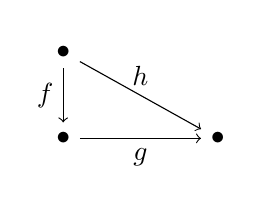
\begin{tikzpicture}[every node/.style={midway}]
      \matrix[column sep={5em,between origins}, row sep={2em}] at (0,0)
      {
        \node(A) {$\bullet$};\\
        \node(B) {$\bullet$}; & \node(C) {$\bullet$}; \\
      };

      \draw[->] (A) -- (B) node[anchor=east] {$f$};
      \draw[->] (B) -- (C) node[anchor=north]  {$g$};
      \draw[->] (A) -- (C) node[anchor=south] {$h$};
    \end{tikzpicture}
  \end{center}
  Primijetimo da objektima nismo dali imena (zato sto nam za ovaj primjer nije
  bitno), ali to ne znaci da su ta tri objekta jednaka. Ako vrijedi
  \begin{align*}
    g \circ f = h
  \end{align*}
  tada kazemo da dijagram \textbf{komutira}.
  Dijagramom zakon asocijativnosti za $f, g, h$ mozemo prikazati kao:
  \begin{center}
    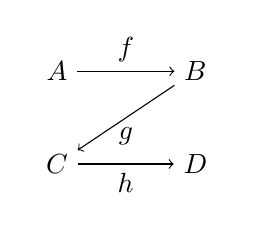
\begin{tikzpicture}[every node/.style={midway}]
      \matrix[column sep={5em,between origins}, row sep={2em}] at (0,0)
      {
        \node(A) {$A$}; & \node(B) {$B$}; \\
        \node(C) {$C$}; & \node(D) {$D$}; \\
      };
      \draw[->] (A) -- (B) node[anchor=south] {$f$};
      \draw[->] (B) -- (C) node[anchor=north] {$g$};
      \draw[->] (C) -- (D) node[anchor=north] {$h$};
    \end{tikzpicture}
  \end{center}


  Kao i u mnogim granama matematike u teoriji kategorija ponekad zelimo
  pokazati da su dvije stvari jednake. Rijetko zelimo pokazati da su dva
  objekta jednaka; cesce cemo pokazivati jednakost strelica i za to cemo
  koristiti tehniku zvanu pracenje dijagrama (en. diagram chasing).
  Dijagram:

  \begin{center}
    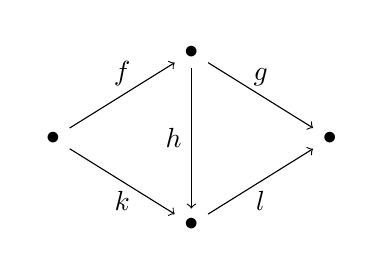
\begin{tikzpicture}[every node/.style={midway}]
      \matrix[column sep={5em,between origins}, row sep={2em}] at (0,0)
      {
        & \node(B) {$\bullet$}; &\\
        \node(A) {$\bullet$}; && \node(C) {$\bullet$}; \\
        & \node(D) {$\bullet$}; & \\
      };
      \draw[->] (A) -- (B) node[anchor=south] {$f$};
      \draw[->] (B) -- (C) node[anchor=south] {$g$};
      \draw[->] (B) -- (D) node[anchor=east] {$h$};
      \draw[->] (A) -- (D) node[anchor=north] {$k$};
      \draw[->] (D) -- (C) node[anchor=north] {$l$};
    \end{tikzpicture}
  \end{center}
  Ima cetiri neimenovana objekta, pet strelica, $f, g, h, k, l$ i pet
  strelica nastalih kompozicijom
  \begin{align*}
    g \circ f, h \circ f, l \circ h \circ f, l \circ h, l \circ k
  \end{align*}
  Primijetimo da neke od tih strelica mogu biti jednake.
  Ovaj dijagram ima tri celije: vanjsku $(f, k, l, g)$, lijevi
  unutarnji trokut $(f, h, k)$ i desni unutarnji trokut $(h, g, l)$.
  Neke od tih celija mogu komutirati:
  \begin{itemize}
      \item lijevi trokut komutira ako vrijedi $h \circ f = k$
      \item desni trokut komutira ako vrijedi $l \circ h = g$
      \item vanjska celija komutira ako vrijedi $g \circ f = l \circ k$
  \end{itemize}
  Pracenje diagrama je proces u kojem pokazemo da neka celija komutira pomocu
  cinjenica da neke druge celije komutiraju i nekih drugih svojstva diagrama

  \begin{primjer} Pokazimo za prijasnji dijagram ako unutarnji trokuti
    komutiraju da tada vanjska celija komutira, tj. da ako vrijedi
    \begin{align*}
      h \circ f = k \qquad  l \circ h = g
    \end{align*}
    data vrijedi:
    \begin{align*}
      g \circ f = l \circ k.
    \end{align*}
    Pokazimo to algebarski:
    \begin{align*}
      g \circ f = (l \circ h) \circ f \overset{(\ref{def:kat_assoc})}{=} l \circ (h \circ f) = l \circ k
    \end{align*}
    Tehnikom pracenja diagrama i primjecivanjem da su neke kompozicije jednake
    imamo:
    \begin{center}
      \begin{tikzpicture}[every node/.style={midway}]
        \matrix[column sep={3em,between origins}, row sep={1em}] at (0,0)
        {
          & \node(B) {$\bullet$}; &&&& \node(E) {$\bullet$}; &&&&&\\
          \node(A) {$\bullet$}; && \node(C) {$\bullet$}; & \node(EQ1) {$=$};
          & \node(D) {$\bullet$}; && \node(G) {$\bullet$}; & \node(EQ2) {$=$};
          & \node(I) {$\bullet$}; && \node(K) {$\bullet$};\\
          &&&&& \node(F) {$\bullet$}; &&&& \node(J) {$\bullet$}; & \\
        };
      \draw[->] (A) -- (B) node[anchor=south] {$f$};
      \draw[->] (B) -- (C) node[anchor=south] {$g$};
      \draw[->] (D) -- (E) node[anchor=south] {$f$};
      \draw[->] (E) -- (F) node[anchor=east] {$h$};
      \draw[->] (F) -- (G) node[anchor=north] {$l$};
      \draw[->] (I) -- (J) node[anchor=north] {$k$};
      \draw[->] (J) -- (K) node[anchor=north] {$l$};
      \end{tikzpicture}
    \end{center}
  \end{primjer}

  Kod jednostavnijih primjera se ne vidi prednost koristenje tehnike dijagrama.
  Pokazimo sad na malo kompliciranijem primjeru kako se tehnikom dijagrama
  intuitivnije moze objasniti komutacija dijagrama.

  \begin{primjer}
    Ako u dijagramu:
    \begin{center}
      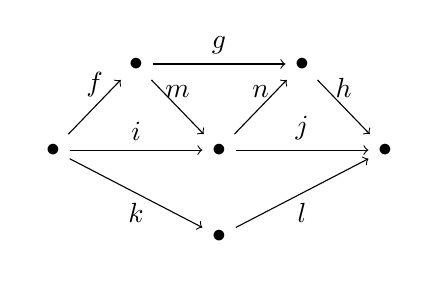
\begin{tikzpicture}[every node/.style={midway}]
        \matrix[column sep={3em,between origins}, row sep={2em}] at (0,0)
        {
          & \node(B) {$\bullet$};&&  \node(C) {$\bullet$}; &\\
          \node(A) {$\bullet$}; && \node(E) {$\bullet$}; && \node(D) {$\bullet$};\\
          && \node(F) {$\bullet$}; &&\\
        };
      \draw[->] (A) -- (B) node[anchor=south] {$f$};
      \draw[->] (B) -- (C) node[anchor=south] {$g$};
      \draw[->] (C) -- (D) node[anchor=south] {$h$};
      \draw[->] (A) -- (E) node[anchor=south] {$i$};
      \draw[->] (E) -- (D) node[anchor=south] {$j$};
      \draw[->] (B) -- (E) node[anchor=south] {$m$};
      \draw[->] (E) -- (C) node[anchor=south] {$n$};
      \draw[->] (A) -- (F) node[anchor=north] {$k$};
      \draw[->] (F) -- (D) node[anchor=north] {$l$};
      \end{tikzpicture}
    \end{center}

    komutiraju cetiri unutarnja trokuta, pokazimo da komutira i vanjska
    celija.

    Cilj nam je pokazati da vrijedi:
    \begin{center}
      $h \circ g \circ f = l \circ k$
    \end{center}
    Algebarski:
    \begin{align*}
      h \circ g \circ f &= h \circ (n \circ m) \circ f = (h \circ n) \circ (m \circ f) =\\
      &= i \circ j = l \circ k\\
    \end{align*}
    Pokazimo to tehnikom pracenja dijagrama.
    \begin{center}
      \begin{tikzpicture}[every node/.style={midway}]
        \matrix[column sep={3em,between origins}, row sep={2em}] at (0,0)
        {
          \node(EQ3) {$\quad$}; && \node(B) {$\bullet$};&&  \node(C) {$\bullet$}; &&
          && \node(B1) {$\bullet$};&&  \node(C1) {$\bullet$}; &\\
          &\node(A) {$\bullet$}; && ; && \node(D) {$\bullet$}; & \node(EQ1) {$=$};
          & \node(A1) {$\bullet$}; && \node(E1) {$\bullet$}; && \node(D1)
          {$\bullet$}; & \node(EQ2) {$=$};\\
        };
      \draw[->] (A) -- (B) node[anchor=south] {$f$};
      \draw[->] (B) -- (C) node[anchor=south] {$g$};
      \draw[->] (C) -- (D) node[anchor=south] {$h$};

      \draw[->] (A1) -- (B1) node[anchor=south] {$f$};
      \draw[->] (C1) -- (D1) node[anchor=south] {$h$};
      \draw[->] (B1) -- (E1) node[anchor=south] {$m$};
      \draw[->] (E1) -- (C1) node[anchor=south] {$n$};

      \end{tikzpicture}
    \end{center}
    \begin{center}
      \begin{tikzpicture}[every node/.style={midway}]
        \matrix[column sep={3em,between origins}, row sep={2em}] at (0,0)
        {
          \node(EQ2) {$=$}; & \node(A) {$\bullet$}; && \node(E) {$\bullet$}; && \node(D)
          {$\bullet$}; & \node(EQ1) {$=$};
          & \node(A1) {$\bullet$}; && && \node(D1) {$\bullet$}; &\\
          &&&&&&&&& \node(F1) {$\bullet$}; &&\\
        };
      \draw[->] (A) -- (E) node[anchor=south] {$i$};
      \draw[->] (E) -- (D) node[anchor=south] {$j$};
      \draw[->] (A1) -- (F1) node[anchor=south] {$k$};
      \draw[->] (F1) -- (D1) node[anchor=south] {$l$};
      \end{tikzpicture}
    \end{center}

  \end{primjer}
  %%%%%%%%%%%%%%%%%%%
  %% Monoik i epik %%
  %%%%%%%%%%%%%%%%%%%
  \newpage
  \section{Monoik i epik}

  \begin{definition}
    U proizvoljnoj kategoriji \category{G} strelicu:
    \begin{align*}
      B \xrightarrow{m} A
    \end{align*}
    Za koju vrijedi da za svaki par strelica
    \begin{align*}
      X \xbigtoto[g]{f} B
    \end{align*}
    vrijedi:
    \begin{align}
      m \circ f = m \circ g \implies f = g
    \end{align}
    Zovemo \textbf{monoik}.
  \end{definition}
  \begin{primjer}
    Neka je \category{G} neka kategorija na skupovima i neka su strelice
    totalne funkcije izmedu skupova.
    Ako je $B \xrightarrow{m} A$ injektivna (kao funkcija) tada je $m$ monoik (kao
    strelica). Pokazimo to.
    Pretpostavimo da vrijedi:
    \begin{align} \label{me:pr:1}
      m \circ f = m \circ g
    \end{align}
    za neki paralelni par strelica
    \begin{align*}
      A \xbigtoto[g]{f} B
    \end{align*}
    Kako su f i g totalne funkcije dovoljno je pokazati da za svaki $x \in X$
    vrijedi:
    \begin{align*}
      f(x) = g(x)
    \end{align*}
    Imamo:
    \begin{align*}
      m(f(x)) = (m \circ f)(x) \overset{(\ref{me:pr:1})}{=} (m \circ g)(x) = m(g(x))
    \end{align*}
    No kako je m injektivna za $a, b \in B$ imamo:
    \begin{align*}
      m(a) = m(b) \implies a = b
    \end{align*}
    pa je $m$ monoik.
    \end{primjer}

  \begin{definition}
    U proizvoljnoj kategoriji \category{G} strelicu:
    \begin{align*}
      A \xrightarrow{e} B
    \end{align*}
    Za koju vrijedi da za svaki par strelica
    \begin{align*}
      B \xbigtoto[g]{f} X
    \end{align*}
    vrijedi:
    \begin{align}
      f \circ e = g \circ e \implies f = g
    \end{align}
    Zovemo \textbf{epik}.
  \end{definition}
  Pokazimo sad na slicnom primjeru kao i prije kako se epik ponasa na
  kategoriji nad skupovima.
  \begin{primjer}
    Neka je \category{G} neka kategorija na skupovima i neka su strelice
    totalne funkcije izmedu skupova.
    Ako je $A \xrightarrow{e} B$ surjektivna (kao funkcija) tada je epik (kao
    strelica).
    Pretpostavimo da vrijedi:
    \begin{align} \label{me:pr:2}
      f \circ e = g \circ e
    \end{align}
    za neki paralelni par strelica
    \begin{align*}
      B \xbigtoto[g]{f} X
    \end{align*}
    Kako su f i g totalne funkcije dovoljno je pokazati da za $x \in X$
    vrijedi:
    \begin{align*}
      f(x) = g(x)
    \end{align*}
    Kako je $e$ surjektivna znamo da za $b \in B$ postoji $a \in A$ takav da
    vrijedi:
    \begin{align*}
      b = e(a)
    \end{align*}
    Imamo
    \begin{align*}
      f(b) = f(e(a)) = (f \circ e)(a) = (g \circ e)(a) = g(e(a)) = g(b)
    \end{align*}
    Pa je $e$ epik.
  \end{primjer}
    Prijasnji primjeri pokazuju da za dovoljno lijepe kategorije vrijedi:
    \begin{center}
      injekcija $\implies$ monoik \qquad surjekcija $\implies$ epik
    \end{center}
    No za neke kategorije "injektivna strelica" ili "surjektivna strelica"
    nemaju smisla, tako da takva intuitivna interpretacija ima smisla za
    "dovoljno lijepe" kategorije. Pravilnije bi bilo gledati na monoik i epik
    kao na strelice koje se mogu "ponistiti" na jednoj strani. Ako pak strelica
    ima jednostrani inverz tada dobivamo posebnu klasu monoika i epika.
    \begin{definition}
      Ako za strelice:
      \begin{align*}
        B \xrightarrow{s} A, \qquad A \xrightarrow{r} B
      \end{align*}
      vrijedi:
      \begin{align*}
        r \circ s = id_B
      \end{align*}
      Tada $s$ nazivamo \textbf{sekcija}, a $r$ \textbf{retrakcija}.
    \end{definition}
    Lako se pokaze da je svaka sekcija monoik i svaka retrakcija epik.
    \begin{definition}
      \textbf{Bimorfizam} je strelica koja je monik i epik.
    \end{definition}
    \begin{definition}
      Za strelicu $A \xrightarrow{f} B$ kazemo da je \textbf{izomorfizam} ako
      postoji strelica $B \xrightarrow{g} A$ takva da vrijedi:
      \begin{align}
        g \circ f = id_A \wedge f \circ g = id_B
      \end{align}
    \end{definition}
    \begin{definition}
      Za dva objekta $A$ i $B$ kazemo da su \textbf{izomorfni} ako postoji izomorfizam
      $A \xrightarrow{} B$.
    \end{definition}

    Lako se pokaze da ukoliko je strelica sekcija i epik ili retrakcija i
    monoik da je tada i izomorfizam.
    Graficki prikazano:
    \begin{center}
    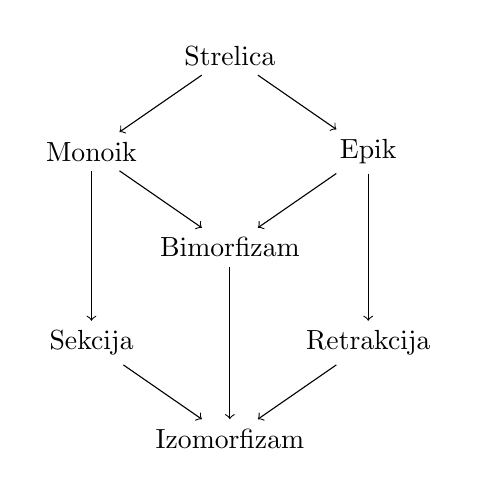
\begin{tikzpicture}[every node/.style={midway}]
      \matrix[column sep={5em,between origins}, row sep={2em}] at (0,0)
      {
        & \node(S) {Strelica}; &\\
        \node(M) {Monoik}; && \node(E) {Epik}; \\
        & \node(B) {Bimorfizam}; & \\
        \node(SM) {Sekcija}; && \node(SE) {Retrakcija};\\
        & \node(I) {Izomorfizam}; & \\
      };
      \draw[->] (S) -- (M) node[anchor=north] {};
      \draw[->] (S) -- (E) node[anchor=north] {};
      \draw[->] (E) -- (SE) node[anchor=north] {};
      \draw[->] (E) -- (B) node[anchor=north] {};
      \draw[->] (M) -- (SM) node[anchor=north] {};
      \draw[->] (M) -- (B) node[anchor=north] {};
      \draw[->] (SM) -- (I) node[anchor=north] {};
      \draw[->] (SE) -- (I) node[anchor=north] {};
      \draw[->] (B) -- (I) node[anchor=north] {};
    \end{tikzpicture}
    \end{center}
  %%%%%%%%%%%%%%%%%%%%%%%%%%%%%%%
  %% Kategorijski konstruktori %%
  %%%%%%%%%%%%%%%%%%%%%%%%%%%%%%%
  \newpage
  \section{Kategorijski konstrukori}
  U ovom poglavlju istrazujemo neke osnovne kategorijske
  konstruktore, tj. objekte koji zadovoljavaju neka pravila definirana u teoriji
  kategorija. Kako u jeziku kategorija ne gledamo unutrasnju strukturu objekata
  svi koncepti moraju biti definirani pomocu relacija izmedu objekata.
  \subsection{Inicijalni i zavrsni objekti}
  \begin{definition}
    Za objekt $S$ u kategoriji \category{G} kazemo da je \textbf{finalni} ako za svaki
    objekt $A$ postoji jedinstvena strelica $A \xrightarrow{} S$.
  \end{definition}
  \begin{definition}
    Za objekt $S$ u kategoriji \category{G} kazemo da je \textbf{inicijalni} ako za svaki
    objekt $A$ postoji jedinstvena strelica $S \xrightarrow{} A$.
  \end{definition}
  \begin{primjer}
    Neka je \category{Set} kategorija skupova i neka je 
    \begin{center}
      $1 = \{x\}$
    \end{center}
    skup s jednim elementom. Za svaki skup $A$ postoji jednistvena strelica
    \begin{center}
      $A \xrightarrow{} 1$
    \end{center}
    (funkcija koja preslikava sve u $x$) pa je $1$ finalni objekt za
    \category{Set}.
    Za svaki skup $A$ postoji jedinstvena strelica
    \begin{center}
      $\emptyset \xrightarrow{} A$
    \end{center}
    (gdje je $\emptyset$ prazan skup) pa je $\emptyset$ inicijalni objekt za
    \category{Set}.
  \end{primjer}
  Kategorija \category{C} moze imati i finalni i inicijalni objekt, a ako ima
  oboje onda oni ne moraju biti isti. Objekt koj je i finalni i inicijalni ponekad
  zovemo \textbf{nulti} objekt. Lako se pokaze da ukoliko kategorija ima dva inicijalna
  objekta da su oni izomorfni pa ima smisla govoriti o inicijalnom objektu
  kategorije (analogno ima smisla govoriti o zavrsnom objektu).
  \subsection{Produkti i koprodukti}
  Produkt u teoriji kategorija je generalizacija Kartezijskog produkta na
  skupovima. Prisjetimo se, ako su $A, B$ skupovi tada je Kartezijev produkt ta
  dva skupa:
  \begin{align*}
    A \times B = \{ (a, b) | a \in A, b \in B\}
  \end{align*}
  Primijetimo da je uz takvu definiciju Kartezijevog produkta prirodno
  definirati dvije projekcije:
  \begin{align*}
    p_A &: A \times B \to A, p_A(a, b) = a\\
    p_B &: A \times B \to B, p_B(a, b) = b\\
  \end{align*}
  Pa na razini kategorija definiramo prvi konstruktor:
  \begin{definition}
    Za $A, B \in Obj_C$ \textbf{grananje prema paru $A, B$} je objekt $X \in
    Obj_C$
    zajedno sa strelicama:
  \begin{center}
    \begin{tikzpicture}[every node/.style={midway}]
      \matrix[column sep={3em,between origins}, row sep={2em}] at (0,0)
      {
        && \node(A) {$A$}; \\
        \node(X) {$X$};\\
        && \node(B) {$B$};\\
      };
      \draw[->] (X) -- (A) node[anchor=south] {};
      \draw[->] (X) -- (B) node[anchor=south] {};
    \end{tikzpicture}
  \end{center}
  \end{definition}
  \begin{definition}
    Za $A, B \in Obj_C$ \textbf{grananje od para $A, B$} je objekt $X \in
    Obj_C$
    zajedno sa strelicama:
  \begin{center}
    \begin{tikzpicture}[every node/.style={midway}]
      \matrix[column sep={3em,between origins}, row sep={2em}] at (0,0)
      {
        \node(A) {$A$}; \\
        && \node(X) {$X$};\\
        \node(B) {$B$};\\
      };
      \draw[->] (A) -- (X) node[anchor=south] {};
      \draw[->] (B) -- (X) node[anchor=south] {};
    \end{tikzpicture}
  \end{center}
  \end{definition}
  Kada ce biti jasno iz konteksta o kojem grananju se raditi, govorit cemo
  samo o grananju. Sada mozemo definirati produkt.
  \begin{definition}
    Neka su $A, B \in Obj_C$. \textbf{Produkt} od $A$ i $B$ je grananje
  \begin{center}
    \begin{tikzpicture}[every node/.style={midway}]
      \matrix[column sep={3em,between origins}, row sep={2em}] at (0,0)
      {
        && \node(A) {$A$}; \\
        \node(S) {$S$};\\
        && \node(B) {$B$};\\
      };
      \draw[->] (S) -- (A) node[anchor=south] {$p_A$};
      \draw[->] (S) -- (B) node[anchor=north] {$p_B$};
    \end{tikzpicture}
  \end{center}
  sa svojstvom da za svako grananje:
  \begin{center}
    \begin{tikzpicture}[every node/.style={midway}]
      \matrix[column sep={3em,between origins}, row sep={2em}] at (0,0)
      {
        && \node(A) {$A$}; \\
        \node(X) {$X$};\\
        && \node(B) {$B$};\\
      };
      \draw[->] (X) -- (A) node[anchor=south] {$f_A$};
      \draw[->] (X) -- (B) node[anchor=north] {$f_B$};
    \end{tikzpicture}
  \end{center}
  postoji jedinstvena strelica $X \xrightarrow{m} S$ takva da dijagram:
  \begin{center}
    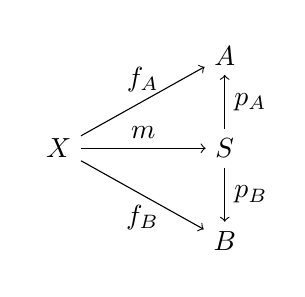
\begin{tikzpicture}[every node/.style={midway}]
      \matrix[column sep={3em,between origins}, row sep={2em}] at (0,0)
      {
        && \node(A) {$A$}; \\
        \node(X) {$X$}; && \node(S) {$S$};\\
        && \node(B) {$B$};\\
      };
      \draw[->] (X) -- (A) node[anchor=south] {$f_A$};
      \draw[->] (X) -- (B) node[anchor=north] {$f_B$};
      \draw[->] (X) -- (S) node[anchor=south] {$m$};
      \draw[->] (S) -- (A) node[anchor=west] {$p_A$};
      \draw[->] (S) -- (B) node[anchor=west] {$p_B$};
    \end{tikzpicture}
  \end{center}
  komutira. Tada $m$ zovemo \textbf{mediator} za grananje na $X$.
  \end{definition}
  Primijetimo dvije stvari:
  \begin{itemize}
    \item produkt nije samo objekt, produkt je objekt i dvije strelice.
    \item mediator je jedinstveni za grananje na $X$
  \end{itemize}
  Analogno definiramo i koprodukt:

  \begin{definition}
    Neka su $A, B \in Obj_C$. \textbf{Koprodukt} od $A$ i $B$ je grananje
  \begin{center}
    \begin{tikzpicture}[every node/.style={midway}]
      \matrix[column sep={3em,between origins}, row sep={2em}] at (0,0)
      {
        \node(A) {$A$}; \\
        && \node(X) {$S$};\\
        \node(B) {$B$};\\
      };
      \draw[->] (A) -- (X) node[anchor=south] {$i_A$};
      \draw[->] (B) -- (X) node[anchor=north] {$i_B$};
    \end{tikzpicture}
  \end{center}
  sa svojstvom da za svako grananje:
  \begin{center}
    \begin{tikzpicture}[every node/.style={midway}]
      \matrix[column sep={3em,between origins}, row sep={2em}] at (0,0)
      {
        \node(A) {$A$}; \\
        && \node(X) {$X$};\\
        \node(B) {$B$};\\
      };
      \draw[->] (A) -- (X) node[anchor=south] {$f_A$};
      \draw[->] (B) -- (X) node[anchor=north] {$f_B$};
    \end{tikzpicture}

  \end{center}
  postoji jedinstvena strelica $S \xrightarrow{m} X$ takva da dijagram:
  \begin{center}
    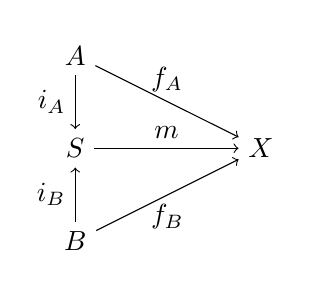
\begin{tikzpicture}[every node/.style={midway}]
      \matrix[column sep={3em,between origins}, row sep={2em}] at (0,0)
      {
        \node(A) {$A$}; \\
        \node(S) {$S$}; && \node(X) {$X$};\\
        \node(B) {$B$};\\
      };
      \draw[->] (A) -- (X) node[anchor=south] {$f_A$};
      \draw[->] (B) -- (X) node[anchor=north] {$f_B$};
      \draw[->] (A) -- (S) node[anchor=east] {$i_A$};
      \draw[->] (B) -- (S) node[anchor=east] {$i_B$};
      \draw[->] (S) -- (X) node[anchor=south] {$m$};
    \end{tikzpicture}
  \end{center}
  komutira.
  \end{definition}
  \begin{definition}
    Za kategoriju \category{C} kazemo da je \textbf{Kartezijeva} (skraceno
    \category{C} je \textbf{CC}) ako:
    \begin{itemize}
      \item sadrzi inicijalni objekt
      \item za svaki par $A, B \in Obj_C$ postoji Kartezijev produkt.
    \end{itemize}
  \end{definition}
  \begin{primjer}
    Za kategoriju \category{Set} smo vec pokazali da sadrzi inicijalni objekt
    $\emptyset$.
    Pokazimo sad da je Kartezijev produkt i produkt u kategorijskom smislu.
    Neka su $A$ i $B$ skupovi.
    Za proizvoljno grananje
    \begin{center}
      \begin{tikzpicture}[every node/.style={midway}]
        \matrix[column sep={3em,between origins}, row sep={2em}] at (0,0)
        {
          && \node(A) {$A$}; \\
          \node(X) {$X$};\\
          && \node(B) {$B$};\\
        };
        \draw[->] (X) -- (A) node[anchor=south] {$f_A$};
        \draw[->] (X) -- (B) node[anchor=north] {$f_B$};
      \end{tikzpicture}
    \end{center}
    na X. Definiramo $X \xrightarrow{m} A \times B$ kao:
    \begin{align*}
      m(x) = (f_A(x), f_B(x))
    \end{align*}
    za $x \in X$. Lako se pokaze da slijedeci diagram komutira:
  \begin{center}
    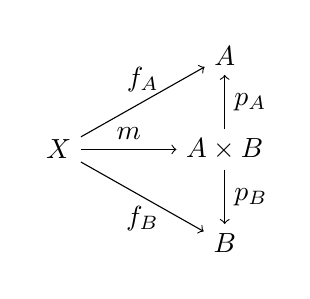
\begin{tikzpicture}[every node/.style={midway}]
      \matrix[column sep={3em,between origins}, row sep={2em}] at (0,0)
      {
        && \node(A) {$A$}; \\
        \node(X) {$X$}; && \node(S) {$A \times B$};\\
        && \node(B) {$B$};\\
      };
      \draw[->] (X) -- (A) node[anchor=south] {$f_A$};
      \draw[->] (X) -- (B) node[anchor=north] {$f_B$};
      \draw[->] (X) -- (S) node[anchor=south] {$m$};
      \draw[->] (S) -- (A) node[anchor=west] {$p_A$};
      \draw[->] (S) -- (B) node[anchor=west] {$p_B$};
    \end{tikzpicture}
  \end{center}
  Ostaje nam pokazati jedinstvenost, tj. da je $m$ jedina takva funkcija.
  Pretpostavimo da postoji neka druga funkcija
  \begin{align*}
    X \xrightarrow{h} A \times B
  \end{align*}
  takva da  vrijedi:
  \begin{align*}
    p_A \circ h = f_A \qquad p_B \circ h = f_B\\
  \end{align*}
  za $x \in X$ imamo:
  \begin{align*}
    h(x) = (p_A(h(x), p_B(h(x))) = ((p_A \circ h )(x), (p_B \circ h)(x)) =
    (f_A(x), f_B(x)) = m(x)
  \end{align*}
  Pa je \category{Set} jedna Kartezijeva kategorija.
  \end{primjer}

  \newpage
  \section*{Literatura}
  \begin{description}
    \item[[2]]
      \url {https://en.wikibooks.org/wiki/Haskell/Category\_theory}
    \item[[3]]
      \url {https://wiki.haskell.org/Type}

    \item[[4]] \label{bib:fast-loose}
      Nils Anders Danielsson, John Hughes, Patrik Jansson, Jeremy Gibbons,
Fast and Loose Reasoning is Morally Correct
\url{http://www.cs.ox.ac.uk/jeremy.gibbons/publications/fast+loose.pdf}
  \end{description}
\end{document}
